\chapter{Conjoin}\label{ch:conjoin}
\section{Introduction}
A finite element analysis can often generate multiple results and/or
restart databases due to model bulk data changes or restarting the
analysis. 

The bulk data changes are caused by element death, element creation,
and surface evolution.  Because the \exo{} database requires a
constant model meta data and bulk data description, the analysis code
must close the current results and restart databases and create new
databases if the model meta data or bulk data change. At the end of
the analysis, there will be multiple database files all describing a
similar model with similar meta data, but with each database
containing a different set of bulk data descriptions of that meta
data.

Another cause of multiple \exo{} databases is when the analysis job is
restarted one or more times.  This is typically the case for
long-running analyses whose total execution time exceeds the maximum
allowed queue time on a compute cluster.  A restart database is
written at the end of each compute segment and then the job is
resubmitted to the compute cluster and is restarted one or more
times. At the end of the analysis, there will be at least one database
for each compute segment and it is often desirable to combine these
databases into a single database for visualization and post processing.

\conjoin{} joins two or more \exo{} databases into a single
database. The input databases should represent the same model geometry
with similar variables. The output database will contain the model
geometry and all of the non-temporally-overlapping results data. If
two databases have overlapping timestep ranges, the timesteps from the
later database will be used. For example, if the first database
contains time data from 0 to 5 seconds, and the second database
contains time data from 4 to 10 seconds; the output database will
contain time data from 0 to 4 seconds from the first database and time
data from 4 to 10 seconds from the second database.  If two nodes have
the same global id and are also colocated, then they are combined to a
single node in the output. Similarly, elements with the same global id
and the same nodal connectivity are combined into a single element in
the output file.

The output database will contain the union of the meta and bulk data
entities (i.e., nodes, elements, element blocks, sidesets, and
nodesets) from each input database. The existence of an entity at a
particular timestep is indicated via a status variable.  For example,
if the first database is the mesh shown in Figure~\ref{fig:cjm1} at
time 0.0 seconds, and the second database is the mesh shown in
Figure~\ref{fig:cjm2} at time 1.0 seconds, then the combined mesh
would be the union of the nodes and elements in the two meshes as
shown in Figure~\ref{fig:cjall}.
\begin{figure}[htp]
\centering
\subfloat[First Database, time 0]{\label{fig:cjm1}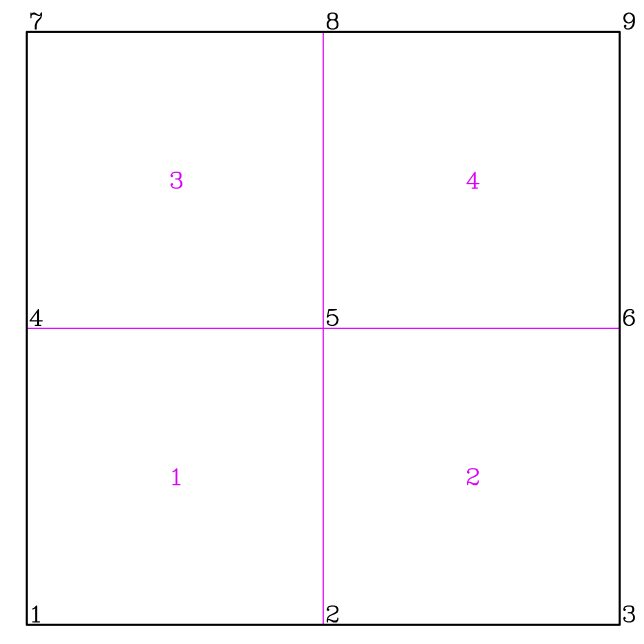
\includegraphics[scale=0.4]{figures/cjm1.png}}
\subfloat[Second Database, time 1]{\label{fig:cjm2}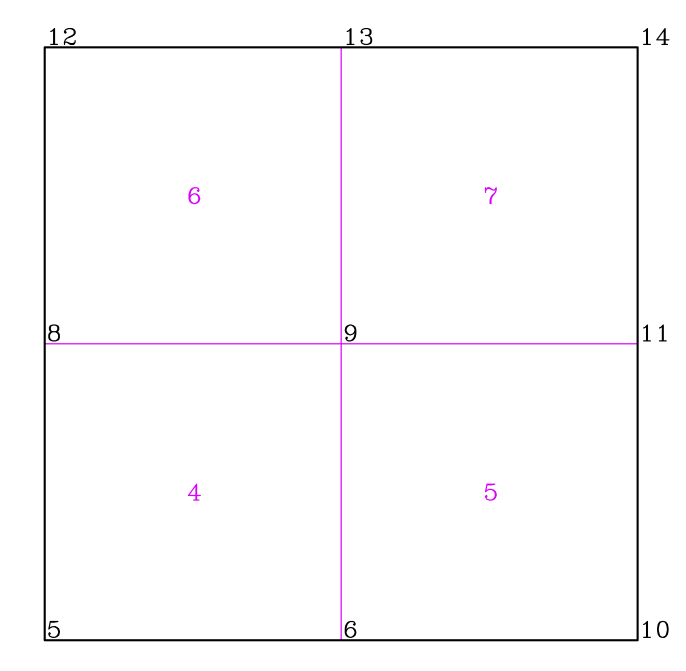
\includegraphics[scale=0.4]{figures/cjm2.png}}
\subfloat[Combined Database, time 0, 1]{\label{fig:cjall}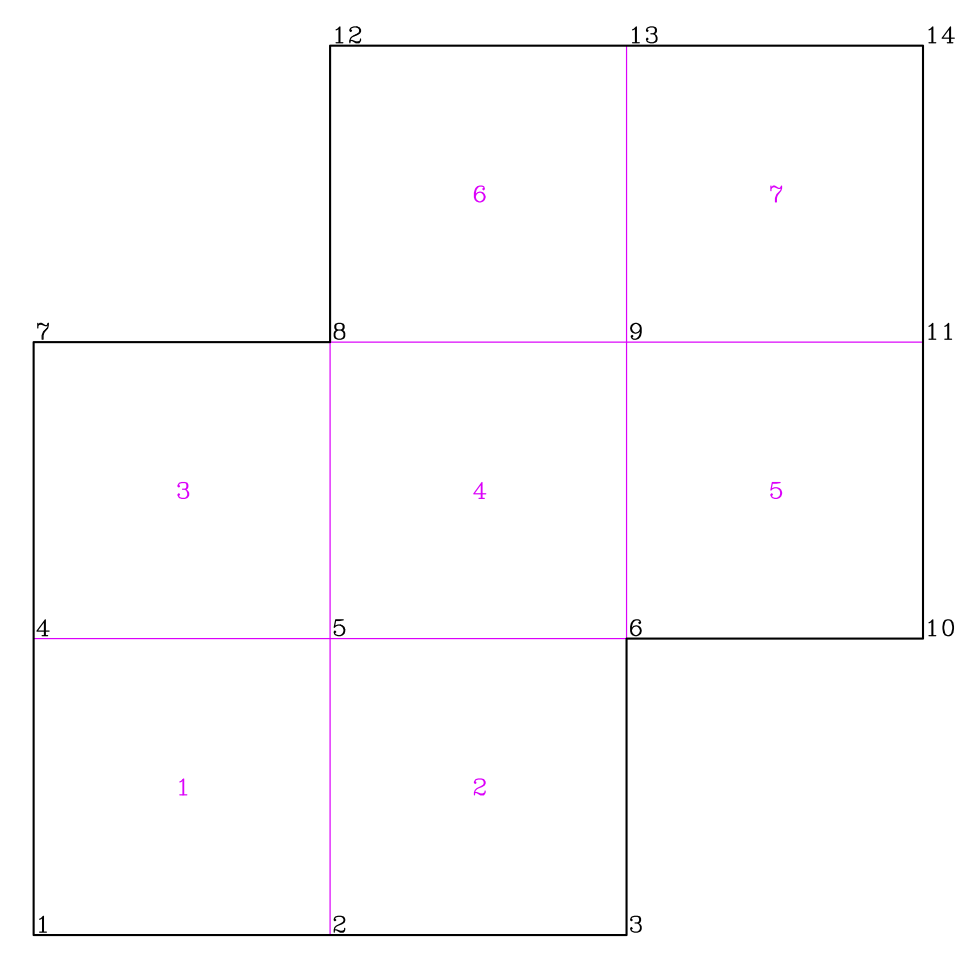
\includegraphics[scale=0.4]{figures/cjall.png}}
\caption{Example Input and Output Meshes for Conjoin}
\end{figure}

The values of the element status variable for each element at each
timestep are shown below.  A status value of 0 indicates that the
element is active and a value of 1 indicates it is inactive. The nodes
have a similar status variable.

\begin{tabular}{l|ccccccc}
\hline
   element        & 1 & 2 & 3 & 4 & 5 & 6 & 7 \\
   status at time 0 & 0 & 0 & 0 & 0 & 1 & 1 & 1 \\
   status at time 1 & 1 & 1 & 1 & 0 & 0 & 0 & 0 \\
\hline
\end{tabular}

The output database will contain the variables that are defined on the
first mesh.  If later databases do not have those variables, then the
data will be zero-filled for those timesteps.  If later databases have
additional variables, they will be ignored.

\section{Invoking \conjoin}
The minimal command line for executing \conjoin{} is:
\begin{syntax}
     conjoin \{list of files to join\}
\end{syntax}
This would create an output mesh named \file{conjoin-out.e} containing
the entities and data from the files listed on the command line.  The
files must be listed in order of increasing time step values.  A nodal
variable named \param{node\_status} and an element variable named
\param{elem\_status} will be added to the variables already existing
on the first file.  The value of the status variables will be 0 to
indicate an active node or element and 1 to indicate an inactive node
or element. 

Several options are available to modify the default behavior of \conjoin{}.

\subsection{Options}
\renewcommand\arraystretch{1.5}
\begin{longtable}{lp{4.0in}}
\param{-help}         & Print this summary and exit  \\
\param{-output <val>} & Name of the output file to create. The
                        default output filename is \file{conjoin-out.e}.  If the specified
			file already exists, it will be overwritten.  \\

\param{-alive\_value <val>}  & Value (1 or 0) which will be used to indicate that an
				element is alive or active. The
				default behavior is that 0 indicates
				alive or active nodes and elements.  \\

\param{-combine\_status\_variables <val>}  & The conjoin elem\_status variable will be combined
                with the specified status variable (val) existing on the mesh.
                Both variables must have the same value (1 or 0) to
		indicate that the element is alive or active. 
                If 1 is alive, then the combined variable is the minimum of the two values.
                If 0 is alive, then the combined variable is the maximum of the two values.
                Use the \param{alive\_value} option to set conjoin's alive value  \\

\param{-element\_status\_variable <val>}  & Element variable name to use as element 
                existence status variable; it must not exist on input files. If specified 
                as NONE, then it will not be written to the output file.
                Default = elem\_status \\

\param{-nodal\_status\_variable <val>}  & Nodal variable name to use as nodal status variable;
		it must not exist on input files. If specified as NONE, 
                then it will not be written to the output file. Default = node\_status  \\

\param{-omit\_nodesets}  & Don't transfer nodesets to output file.  \\
\param{-omit\_sidesets}  & Don't transfer sidesets to output file.  \\
\param{-gvar <val>} & Comma-separated list of global variables to be
		joined or ALL or NONE.  The default behavior is that all global
		variables will be written to the output file.\\
\param{-evar <val>} & Comma-separated list of element variables to be joined or ALL or NONE.
                Variables can be limited to certain blocks by appending a
                colon followed by the block id.  For example,
		\param{-evar sigxx:10:20} would result in the variable
		\param{sigxx} would be written for element blocks with
		id 10 and 20. The default behavior is that all element
		variables will be written to the output file.  \\
\param{-nvar <val>} & Comma-separated list of nodal variables to be
		joined or ALL or NONE. The default behavior is that all nodal 
		variables will be written to the output file. \\
\param{-nsetvar <val>} & Comma-separated list of nodeset variables to
		be joined or ALL or NONE.  The default behavior is that all nodeset 
		variables will be written to the output file.\\
\param{-ssetvar <val>} & Comma-separated list of sideset variables to
		be joined or ALL or NONE.  The default behavior is that all sideset 
		variables will be written to the output file.\\
\param{-debug <val>}  & Debug level (values are or'd)\par
	\begin{tabular}{l@{ = }l}
                  1 & timing information.\\
                  4 & Verbose Element block information.\\
                  8 & Check consistent nodal coordinates between parts.\\
                 16 & Verbose Sideset information.\\
                 32 & Verbose Nodeset information.\\
                 64 & put exodus library into verbose mode.\\
                128 & Check consistent global field values between parts.  \\
	\end{tabular}\\
\param{-width <val>}  & Width of output screen, default = 80  \\
\param{-version}      & Print version and exit  \\
\param{-copyright}  & Show copyright and license data.  \\
\end{longtable}

When \conjoin{} is invoked, it will parse the user-specified options from
the command line and it will also see if the environment variable
\param{CONJOIN\_OPTIONS} exists.  If the variable exists, then it will be
parsed first followed by the parsing of the options on the command line.

\section{Example}
The output below shows the results of running the following command:
\begin{syntax}
	conjoin -output adapt.e adaptBox.e*
\end{syntax}

The first section of the output shows the code version followed by some
information showing the map from part number to filename. In this case
there are 6 parts which will be joined.

\begin{verbatim}
conjoin
        (A code for sequentially appending Exodus II databases. Supercedes conex and conex2.)
        (Version: 1.2.1) Modified: 2011/01/12
Part 1: 'adaptBox.e'
Part 2: 'adaptBox.e-s0002'
Part 3: 'adaptBox.e-s0003'
Part 4: 'adaptBox.e-s0004'
Part 5: 'adaptBox.e-s0005'
Part 6: 'adaptBox.e-s0006'
\end{verbatim}
\sectionline
The next section of the output shows the output filename
(\file{adapt.e} in this example), and gives a summary of the output
mesh showing the entity counts and the variable summary.
\begin{verbatim}
Output:   'adapt.e'
IO Word size is 8 bytes.
 Title: Default Sierra Title

 Number of coordinates per node       =        3
 Number of nodes                      =      151
 Number of elements                   =       84
 Number of element blocks             =        1

 Number of nodal point sets           =        0
 Number of element side sets          =        2


Reading and Writing element connectivity & attributes

Wrote coordinate names...
Wrote coordinate information...
Found 7 global variables.
        ExternalEnergy  InternalEnergy  KineticEnergy   Momentum_x      
        Momentum_y      Momentum_z      TIMESTEP        

Found 7 nodal variables.
        displ_x      displ_y      displ_z      vel_x        vel_y        
        vel_z        node_status  

Found 7 element variables.
        stress_xx    stress_yy    stress_zz    stress_xy    stress_yz    
        stress_zx    elem_status  
\end{verbatim}
\sectionline

The last section shows the progress of transferring the transient data
to the output mesh.  For each timestep, the output shows the part from
which the data is being read and which timestep within that part is
being used.  It also show how many elements are active in that part
and an estimate of how long it will take to finish transferring the
data.  Figures~\ref{fig:cjex1} to~\ref{fig:cjex4} show four views of
the output mesh.

\begin{verbatim}
Step  1/11, time 0.0000e+00 (Part 1/6, step 1)  Active Elem:  4  [  9%, Elapsed=0.0s, ETA=0.0s]
Step  2/11, time 5.0000e-01 (Part 1/6, step 2)  Active Elem:  4  [ 18%, Elapsed=0.0s, ETA=0.0s]
Step  3/11, time 1.0000e+00 (Part 2/6, step 1)  Active Elem: 11  [ 27%, Elapsed=0.0s, ETA=0.0s]
Step  4/11, time 1.2500e+00 (Part 3/6, step 1)  Active Elem: 74  [ 36%, Elapsed=0.0s, ETA=0.0s]
Step  5/11, time 1.5000e+00 (Part 3/6, step 2)  Active Elem: 74  [ 45%, Elapsed= <1s, ETA= <1s]
Step  6/11, time 1.7500e+00 (Part 4/6, step 1)  Active Elem: 46  [ 55%, Elapsed= <1s, ETA= <1s]
Step  7/11, time 2.0000e+00 (Part 4/6, step 2)  Active Elem: 46  [ 64%, Elapsed= <1s, ETA= <1s]
Step  8/11, time 2.5000e+00 (Part 4/6, step 3)  Active Elem: 46  [ 73%, Elapsed= <1s, ETA= <1s]
Step  9/11, time 3.0000e+00 (Part 5/6, step 1)  Active Elem: 18  [ 82%, Elapsed= <1s, ETA= <1s]
Step 10/11, time 3.5000e+00 (Part 6/6, step 1)  Active Elem:  4  [ 91%, Elapsed= <1s, ETA= <1s]
Step 11/11, time 4.0000e+00 (Part 6/6, step 2)  Active Elem:  4  [100%, Elapsed= <1s, ETA=0.0s]
******* END *******
\end{verbatim}
\begin{figure}[ht]
\centering
\subfloat[Time 0.0]{\label{fig:cjex1}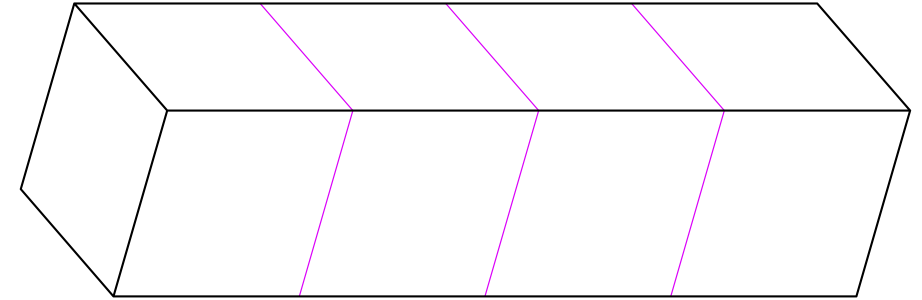
\includegraphics[scale=0.25]{figures/cjex1s.png}}
\subfloat[Time 1.0]{\label{fig:cjex2}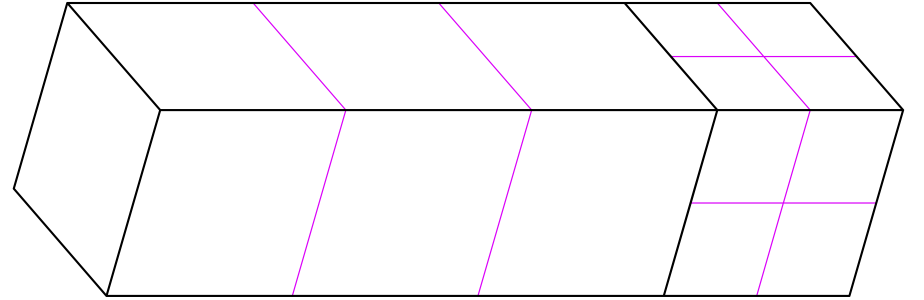
\includegraphics[scale=0.25]{figures/cjex2s.png}}\\
\subfloat[Time 1.5]{\label{fig:cjex3}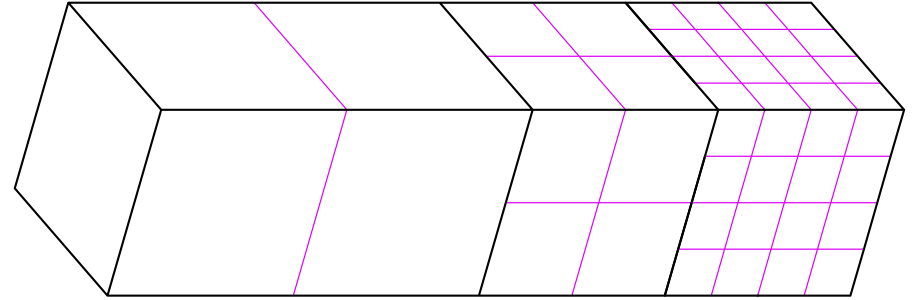
\includegraphics[scale=0.25]{figures/cjex3s.png}}
\subfloat[Time 2.5]{\label{fig:cjex4}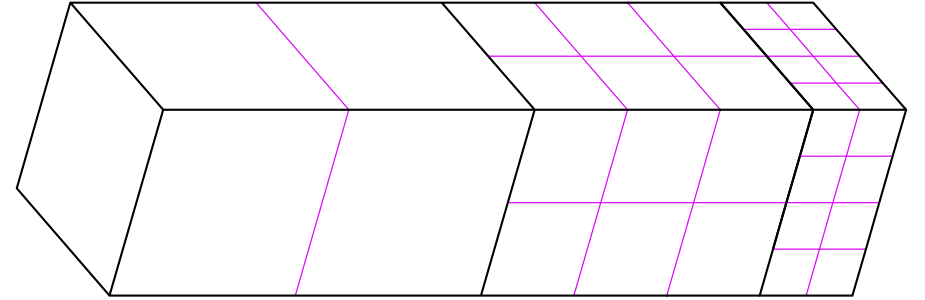
\includegraphics[scale=0.25]{figures/cjex4s.png}}
\caption{Example Output Mesh from Conjoin}
\end{figure}

\section{Related Codes}
\conjoin{} replaces the functionality of the
\code{conex}\cite{bib:conex} code.  \conjoin{} provides a superset of
the \code{conex} functionality and is also much faster. \conjoin{}
also supports nodeset and sideset variables and the naming of element
blocks, nodesets, and sidesets which is not supported by
\code{conex}. The input mesh databases to \code{Conex} are required to
have the exact same bulk data which limits its use for adaptive
analyses and other analyses which have varying numbers of active and
inactive nodes and elements.  \code{Conex} is no longer actively
supported. 
